\documentclass[tikz,border=0pt]{standalone}

\usepackage[T1]{fontenc}
\usepackage{newtxtext,newtxmath}
% newtxmath defines \Bbbk before amssymb on this TeX Live build.
\let\Bbbk\relax
\usepackage{amsmath,amssymb,bm}
\usepackage{tikz}
\usepackage{pgfplots}

\usetikzlibrary{
  arrows.meta,
  positioning,
  fit,
  calc,
  backgrounds,
  shapes.geometric,
  shapes.multipart,
  matrix,
  decorations.pathreplacing
}

\pgfplotsset{compat=1.18}

\definecolor{FigTeal}{HTML}{539F97}
\definecolor{FigBlue}{HTML}{6C7AAD}
\definecolor{FigRose}{HTML}{BE7A7A}
\definecolor{FigDark}{HTML}{252525}
\definecolor{FigGrid}{HTML}{E7EBEF}
\definecolor{FigNeutral}{HTML}{F5F4F0}
\definecolor{FigLightTeal}{HTML}{DDECEA}
\definecolor{FigLightBlue}{HTML}{E3E6F0}
\definecolor{FigLightRose}{HTML}{F0DFDF}

\newcommand{\panelfont}{\fontsize{9.0}{10.2}\selectfont\bfseries}
\newcommand{\grouptitlefont}{\fontsize{8.4}{9.4}\selectfont\bfseries}
\newcommand{\boxtitlefont}{\fontsize{7.9}{8.8}\selectfont\bfseries}
\newcommand{\normalfontsmall}{\fontsize{7.2}{8.0}\selectfont}
\newcommand{\eqfont}{\fontsize{7.2}{8.0}\selectfont}
\newcommand{\smallfont}{\fontsize{6.9}{7.6}\selectfont}
\newcommand{\labelfontsmall}{\fontsize{6.9}{7.6}\selectfont}

\tikzset{
  panel/.style={
    rounded corners=3pt,
    draw=FigGrid,
    fill=FigNeutral,
    line width=0.65pt
  },
  basebox/.style={
    rounded corners=2pt,
    draw=FigDark,
    fill=white,
    line width=0.75pt,
    align=center,
    inner sep=3.5pt
  },
  statebox/.style={
    basebox,
    draw=FigBlue,
    fill=FigLightBlue
  },
  policybox/.style={
    basebox,
    draw=FigBlue,
    fill=FigLightBlue
  },
  actionbox/.style={
    basebox,
    draw=gray!75!black,
    fill=white
  },
  envbox/.style={
    basebox,
    draw=FigTeal,
    fill=FigLightTeal
  },
  rewardbox/.style={
    basebox,
    draw=FigRose,
    fill=FigLightRose
  },
  updatebox/.style={
    basebox,
    draw=FigRose,
    fill=FigLightRose
  },
  neutralbox/.style={
    basebox,
    draw=gray!75!black,
    fill=white
  },
  scenarioblue/.style={
    basebox,
    draw=FigBlue,
    fill=FigLightBlue
  },
  scenarioteal/.style={
    basebox,
    draw=FigTeal,
    fill=FigLightTeal
  },
  scenariorose/.style={
    basebox,
    draw=FigRose,
    fill=FigLightRose
  },
  dataflow/.style={
    -{Latex[length=2.0mm,width=1.2mm]},
    draw=FigDark,
    line width=0.9pt
  },
  feedback/.style={
    -{Latex[length=2.0mm,width=1.2mm]},
    draw=FigBlue,
    line width=0.85pt
  },
  trainflow/.style={
    -{Latex[length=2.0mm,width=1.2mm]},
    draw=FigRose,
    dashed,
    line width=0.8pt
  },
  auxflow/.style={
    -{Latex[length=1.8mm,width=1.1mm]},
    draw=gray!75!black,
    line width=0.75pt
  },
  arrowlabel/.style={
    fill=white,
    inner sep=1.1pt,
    font=\labelfontsmall,
    text=FigDark
  }
}

\begin{document}
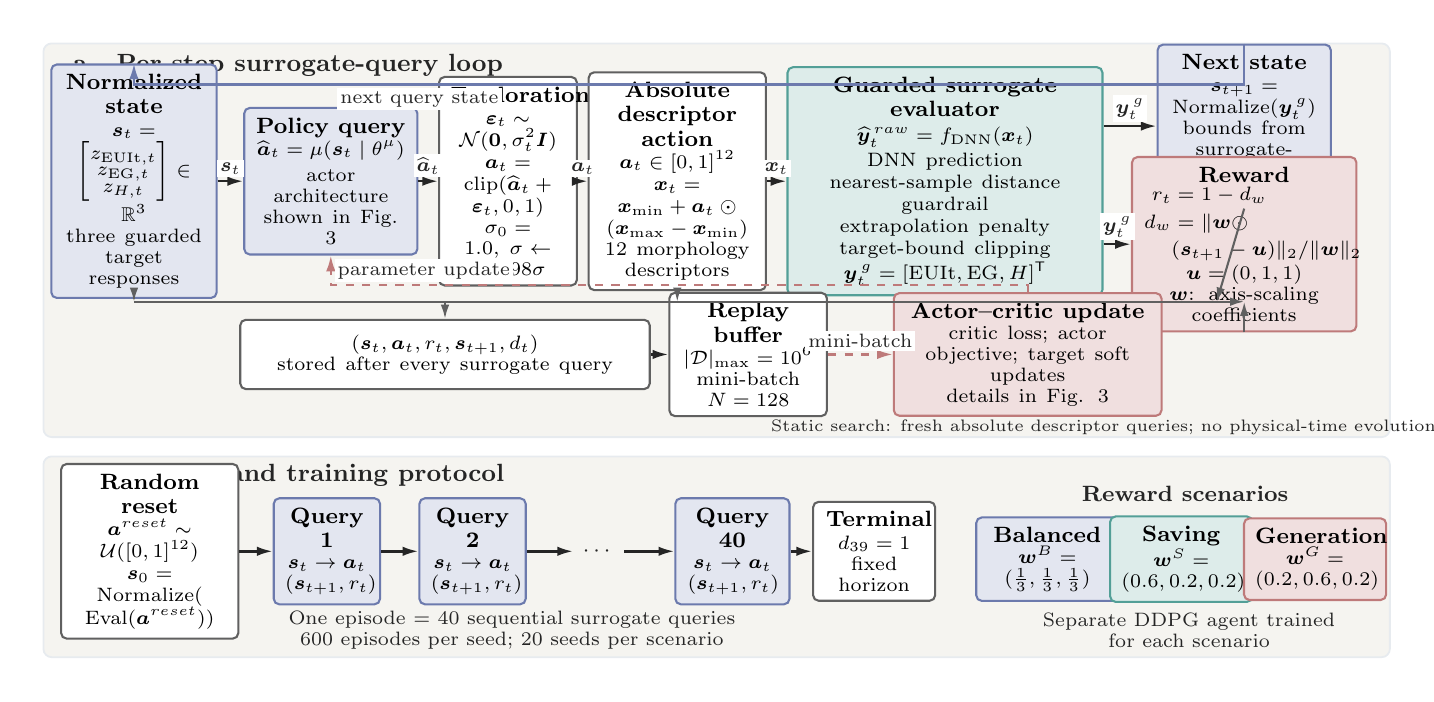
\begin{tikzpicture}[x=1cm,y=1cm]
\path[use as bounding box] (0,0) rectangle (17.5,8.2);

\node[panel, minimum width=17.1cm, minimum height=5.0cm] (panela) at (8.75,5.50) {};
\node[panel, minimum width=17.1cm, minimum height=2.55cm] (panelb) at (8.75,1.48) {};
\node[anchor=west, font=\panelfont, text=FigDark] at (0.45,7.72) {a\quad Per-step surrogate-query loop};
\node[anchor=west, font=\panelfont, text=FigDark] at (0.45,2.52) {b\quad Episode and training protocol};

\node[statebox, minimum width=2.1cm, minimum height=1.45cm, text width=1.82cm] (state) at (1.35,6.25) {%
  \begin{minipage}{1.78cm}\centering
  {\boxtitlefont Normalized state\par}
  {\eqfont
  $\bm s_t=
  \begin{bmatrix}
  z_{\mathrm{EUIt},t}\\[-2pt]
  z_{\mathrm{EG},t}\\[-2pt]
  z_{H,t}
  \end{bmatrix}
  \in\mathbb R^3$\par}
  {\smallfont three guarded target responses\par}
  \end{minipage}
};

\node[policybox, minimum width=2.2cm, minimum height=1.45cm, text width=1.94cm] (policy) at (3.85,6.25) {%
  \begin{minipage}{1.90cm}\centering
  {\boxtitlefont Policy query\par}
  {\eqfont
  $\widehat{\bm a}_t=\mu(\bm s_t\mid\theta^\mu)$\par}
  \vspace{2pt}
  {\smallfont actor architecture shown in Fig. 3\par}
  \end{minipage}
};

\node[neutralbox, minimum width=1.75cm, minimum height=1.45cm, text width=1.50cm] (explore) at (6.10,6.25) {%
  \begin{minipage}{1.46cm}\centering
  {\boxtitlefont Exploration\par}
  {\eqfont
  $\bm\varepsilon_t\sim\mathcal N(\bm 0,\sigma_t^2\bm I)$\par
  $\bm a_t=\operatorname{clip}(\widehat{\bm a}_t+\bm\varepsilon_t,0,1)$\par}
  {\smallfont $\sigma_0=1.0,\;\sigma\leftarrow0.9998\sigma$\par}
  \end{minipage}
};

\node[actionbox, minimum width=2.25cm, minimum height=1.45cm, text width=1.98cm] (action) at (8.25,6.25) {%
  \begin{minipage}{1.94cm}\centering
  {\boxtitlefont Absolute descriptor action\par}
  {\eqfont
  $\bm a_t\in[0,1]^{12}$\par
  $\bm x_t=\bm x_{\min}+\bm a_t\odot(\bm x_{\max}-\bm x_{\min})$\par}
  {\smallfont 12 morphology descriptors\par}
  \end{minipage}
};

\node[envbox, minimum width=4.0cm, minimum height=2.15cm, text width=3.68cm] (evaluator) at (11.65,6.25) {%
  \begin{minipage}{3.64cm}\centering
  {\boxtitlefont Guarded surrogate evaluator\par}
  \vspace{1pt}
  {\eqfont $\widehat{\bm y}^{\,raw}_t=f_{\mathrm{DNN}}(\bm x_t)$\par}
  \vspace{1pt}
  {\normalfontsmall DNN prediction\par}
  {\normalfontsmall nearest-sample distance guardrail\par}
  {\normalfontsmall extrapolation penalty\par}
  {\normalfontsmall target-bound clipping\par}
  \vspace{1pt}
  {\eqfont $\bm y^{\,g}_t=[\mathrm{EUIt},\mathrm{EG},H]^\mathsf T$\par}
  \end{minipage}
};

\node[statebox, minimum width=2.2cm, minimum height=1.15cm, text width=1.90cm] (nextstate) at (15.45,6.95) {%
  \begin{minipage}{1.86cm}\centering
  {\boxtitlefont Next state\par}
  {\eqfont $\bm s_{t+1}=\operatorname{Normalize}(\bm y^{\,g}_t)$\par}
  {\smallfont bounds from surrogate-training domain\par}
  \end{minipage}
};

\node[rewardbox, minimum width=2.85cm, minimum height=1.35cm, text width=2.58cm] (reward) at (15.45,5.45) {%
  \begin{minipage}{2.54cm}\centering
  {\boxtitlefont Reward\par}
  {\eqfont
  $\begin{aligned}
  r_t&=1-d_w\\[-1pt]
  d_w&=\|\bm w\odot\\[-1pt]
  &(\bm s_{t+1}-\bm u)\|_2/\|\bm w\|_2
  \end{aligned}$\par
  $\bm u=(0,1,1)$\par}
  {\smallfont $\bm w$: axis-scaling coefficients\par}
  \end{minipage}
};

\node[neutralbox, minimum width=5.2cm, minimum height=0.88cm, text width=4.86cm] (transition) at (5.30,4.05) {%
  \begin{minipage}{4.82cm}\centering
  {\eqfont $(\bm s_t,\bm a_t,r_t,\bm s_{t+1},d_t)$\par}
  {\smallfont stored after every surrogate query\par}
  \end{minipage}
};

\node[neutralbox, minimum width=2.0cm, minimum height=0.88cm, text width=1.72cm] (buffer) at (9.15,4.05) {%
  \begin{minipage}{1.68cm}\centering
  {\boxtitlefont Replay buffer\par}
  {\eqfont $|\mathcal D|_{\max}=10^6$\par}
  {\smallfont mini-batch $N=128$\par}
  \end{minipage}
};

\node[updatebox, minimum width=3.4cm, minimum height=0.88cm, text width=3.08cm] (update) at (12.70,4.05) {%
  \begin{minipage}{3.04cm}\centering
  {\boxtitlefont Actor--critic update\par}
  {\smallfont critic loss; actor objective; target soft updates\par}
  {\smallfont details in Fig. 3\par}
  \end{minipage}
};

\node[font=\fontsize{6.2}{6.7}\selectfont, text=FigDark, align=center] at (13.70,3.13)
  {Static search: fresh absolute descriptor queries; no physical-time evolution.};

\draw[dataflow] (state.east) -- node[arrowlabel, above=1pt] {$\bm s_t$} (policy.west);
\draw[dataflow] (policy.east) -- node[arrowlabel, above=1pt] {$\widehat{\bm a}_t$} (explore.west);
\draw[dataflow] (explore.east) -- node[arrowlabel, above=1pt] {$\bm a_t$} (action.west);
\draw[dataflow] (action.east) -- node[arrowlabel, above=1pt] {$\bm x_t$} (evaluator.west);
\draw[dataflow] (evaluator.east |- nextstate.west) -- node[arrowlabel, above=1pt] {$\bm y_t^{\,g}$} (nextstate.west);
\draw[dataflow] (evaluator.east |- reward.west) -- node[arrowlabel, above=1pt] {$\bm y_t^{\,g}$} (reward.west);
\draw[feedback] (nextstate.north) |- (8.60,7.48) -| node[arrowlabel, near start, below=1pt] {next query state} (state.north);

\coordinate (busL) at (1.35,4.72);
\coordinate (busR) at (15.45,4.72);
\draw[auxflow] (state.south) -- (1.35,4.72);
\draw[auxflow] (action.south) -- (8.25,4.72);
\draw[auxflow] (reward.south) -- (15.45,4.72);
\draw[auxflow] (nextstate.south) -- (15.10,4.72);
\draw[auxflow] (busL) -- (busR);
\draw[auxflow] (5.30,4.72) -- (transition.north);
\draw[dataflow] (transition.east) -- (buffer.west);
\draw[trainflow] (buffer.east) -- node[arrowlabel, above=1pt] {mini-batch} (update.west);
\draw[trainflow] (update.north) |- (8.15,4.93) -| node[arrowlabel, near end, right=1pt] {parameter update} (policy.south);

\node[neutralbox, minimum width=2.25cm, minimum height=0.95cm, text width=1.98cm] (reset) at (1.55,1.55) {%
  \begin{minipage}{1.94cm}\centering
  {\boxtitlefont Random reset\par}
  {\eqfont $\bm a^{reset}\sim\mathcal U([0,1]^{12})$\par
  $\bm s_0=\operatorname{Normalize}($\par
  $\operatorname{Eval}(\bm a^{reset}))$\par}
  \end{minipage}
};
\node[statebox, minimum width=1.35cm, minimum height=0.82cm, text width=1.10cm] (q1) at (3.80,1.55) {%
  \begin{minipage}{1.06cm}\centering
  {\boxtitlefont Query 1\par}
  {\smallfont $\bm s_t\to\bm a_t$\par $(\bm s_{t+1},r_t)$\par}
  \end{minipage}
};
\node[statebox, minimum width=1.35cm, minimum height=0.82cm, text width=1.10cm] (q2) at (5.65,1.55) {%
  \begin{minipage}{1.06cm}\centering
  {\boxtitlefont Query 2\par}
  {\smallfont $\bm s_t\to\bm a_t$\par $(\bm s_{t+1},r_t)$\par}
  \end{minipage}
};
\node[font=\grouptitlefont, text=FigDark] (dots) at (7.25,1.55) {$\cdots$};
\node[statebox, minimum width=1.45cm, minimum height=0.82cm, text width=1.18cm] (q40) at (8.95,1.55) {%
  \begin{minipage}{1.14cm}\centering
  {\boxtitlefont Query 40\par}
  {\smallfont $\bm s_t\to\bm a_t$\par $(\bm s_{t+1},r_t)$\par}
  \end{minipage}
};
\node[neutralbox, minimum width=1.55cm, minimum height=0.82cm, text width=1.26cm] (terminal) at (10.75,1.55) {%
  \begin{minipage}{1.22cm}\centering
  {\boxtitlefont Terminal\par}
  {\eqfont $d_{39}=1$\par}
  {\smallfont fixed horizon\par}
  \end{minipage}
};
\draw[dataflow] (reset.east) -- (q1.west);
\draw[dataflow] (q1.east) -- (q2.west);
\draw[dataflow] (q2.east) -- (dots.west);
\draw[dataflow] (dots.east) -- (q40.west);
\draw[dataflow] (q40.east) -- (terminal.west);
\node[font=\smallfont, text=FigDark, align=center] at (6.15,0.55) {One episode = 40 sequential surrogate queries\\600 episodes per seed; 20 seeds per scenario};

\node[font=\grouptitlefont, text=FigDark] at (14.70,2.28) {Reward scenarios};
\node[scenarioblue, minimum width=1.75cm, minimum height=0.82cm, text width=1.56cm] (balanced) at (12.95,1.45) {%
  \begin{minipage}{1.52cm}\centering
  {\boxtitlefont Balanced\par}
  {\smallfont $\bm w^B=(\tfrac13,\tfrac13,\tfrac13)$\par}
  \end{minipage}
};
\node[scenarioteal, minimum width=1.75cm, minimum height=0.82cm, text width=1.56cm] (saving) at (14.65,1.45) {%
  \begin{minipage}{1.52cm}\centering
  {\boxtitlefont Saving\par}
  {\smallfont $\bm w^S=$\par $(0.6,0.2,0.2)$\par}
  \end{minipage}
};
\node[scenariorose, minimum width=1.75cm, minimum height=0.82cm, text width=1.56cm] (generation) at (16.35,1.45) {%
  \begin{minipage}{1.52cm}\centering
  {\boxtitlefont Generation\par}
  {\smallfont $\bm w^G=$\par $(0.2,0.6,0.2)$\par}
  \end{minipage}
};
\node[font=\smallfont, text=FigDark, align=center] at (14.75,0.55) {Separate DDPG agent trained\\for each scenario};

\end{tikzpicture}
\end{document}
